 \documentclass[12pt]{article}
\usepackage[a4paper, total={6in, 8in}]{geometry}
\usepackage[utf8]{inputenc}
\usepackage[round]{natbib}
\usepackage{graphicx}
\usepackage{dblfloatfix}    % To enable figures at the bottom of page
\usepackage{rotating}
\usepackage{tikz}
\usepackage{authblk}
\usepackage{booktabs, tabularx}
\usepackage{amsmath}
\usepackage[input-decimal-markers=.]{siunitx}
\usepackage[english]{babel}
\usepackage{pdflscape}
\usepackage{setspace} \doublespacing
\usepackage{dcolumn,caption}
\usepackage{array, threeparttable} % to add footnotes to the tables
\setlength{\emergencystretch}{3em}
\captionsetup{skip=0.333\baselineskip}
\newcolumntype{d}[1]{D{.}{.}{#1}}
\newcommand\mc[1]{\multicolumn{1}{@{}c@{}}{#1}} % handy shortcut macro

\begin{document}

\title{Online skills endorsement and start-up funding: evidence from digital new ventures in the greater Paris}
\date{\vspace{-3ex}}
\author{Arnauld Bessagnet \\ \footnotesize{LEREPS – Sciences-Po Toulouse, University of Toulouse – France} \\}

\maketitle \vspace{-1,5em}

\begin{abstract}
\noindent
Entrepreneurship research and signaling theory suggest that a start-up team human capital signals its quality to investors, affecting their ability to secure financing. Yet, no studies, to our knowledge, have explored the signaling effect of online skills endorsement — a human capital peer-reviewed measure available on professional social networks considered as a reliable criteria in order to judge a person’s knowledge authority — and its impact on early-stage venture funding. This study, based on 439 French start-ups, investigates this relationship. Results indicate that investors prefer start-up teams with either a high level of skills or a high level of variety of skills, but only some at once. We discuss these findings' implications for entrepreneurship and new venture financing literature. \newline

\begin{obeylines}
\noindent \footnotesize{}{\textbf{Keywords:} skills endorsement, entrepreneurship, fundraising, start-up teams, variety}
\noindent \footnotesize{\textbf{JEL Classification:} L22, L26, L85}
\end{obeylines}

\end{abstract}

\clearpage
\section{Introduction}

Which start-up teams are funded and why are recurring themes in contemporary economic and entrepreneurial literature \citep{baum2004picking, beckman2007early, bernstein2017attracting, franke2006you, franke2008venture, kaplan2009should, plummer2016better, shane2002network}. In entrepreneurship literature, start-up teams, defined as groups of individuals exhibiting attributes such as equity ownership, decision-making autonomy, and entitativeness \citep{knight2020start}, are recognized as essential agents for the development of cities, regions, and countries due to their role in firm creation and growth \citep{audretsch2001linking, autio2016entrepreneurship}. Acquiring financial resources is a key factor for their survival and expansion \citep{rosenbusch2013does}, thus making the determinants of attracting such resources of great interest to researchers, practitioners, and policy makers \citep{EUcommission2015digital}.

The literature underlines the complex impact of start-up team composition on investor decisions \citep{ghassemiautomated}. Start-up teams qualities such as founders' education, prior work experiences or entrepreneurial experiences \citep{shane2002network, hsu2007experienced}, and their relationships with investors and partners \citep{huang2017resources}, serve as quality signals for obtaining financial resources. While these studies yielded important insights, this approach is problematic as investors nowadays draw on a wide range of other signals to assess the relevance of investing in a start-up team. For instance, \citet{banerji2019startup} found that founders' number of followers on their LinkedIn profiles was the strongest predictor of the amount of funds raised by new ventures. In the same vein, based on data available on Kickstarter crowdfunding website, \citet{mollick2014dynamics} evidences that founders' Facebook connections help equity crowdfunding success and \citet{courtney2017resolving} show how third party online endorsements help firm attract fundings.

In the business literature, skill endorsement is considered a socially constructed online reputation and a way of self-presentation through which job seekers brand themselves to potential recruiters \citep{rapanta2017linkedin}. Concretely, it permits users to tag themselves with topics representing their area of expertise and have their connections provide social proof of their competence in that topic. For example, some social networks, such as LinkedIn and ResearchGate, allow users to endorse specific skills that are associated with authority and social credit \citep{perez2016endorsement, wu2018analysis}. In entrepreneurship studies, researchers have considered online skills endorsements data as valuable information for entrepreneurial studies and consider it as a reliable criteria in order to judge a person’s knowledge \citep{reese2020should, sako2020scaling}. Nonetheless, research on the potential signaling effects of online skills endorsement on early stage resource acquisition was left out by researchers.

This study seeks to fill this gap by examining the role of online skills endorsement in resource acquisition during the early stages of a start-up teams. Drawing on the theory of signaling, we explore how online skills endorsement - a human capital peer-reviewed data available on professional social networks considered as a reliable criteria in order to judge a person’s knowledge authority - can influence the ability of start-up teams to acquire financial resources from investors \citep{rapanta2017linkedin}. To do so, we use data from a sample of 439 french digital new ventures and human capital data on their start-up teams. We constructed a unique dataset that includes online reputation start-up teams data that can be classified into "human capital investments" (i.e., common traditional signals used by investors such as years of education, professional experience, and previous founding experience) and "outcomes of human capital" (i.e., skills, abilities and knowledge) of start-up teams \citep{marvel2016human}. We focus on the later as our main independent variable and use the former as moderating variables. We analyze our statement in two stages. First, we examine the relationship between the level of online skills endorsement of start-up teams and its impact on capital acquisitions in early-stage investment. Secondly, drawing from the cognitive distance model \citep{nooteboom2007optimal} and the cybernetics principles of requisite variety applied to the entrepreneurship literature \citep{ashby1957introduction, harrison2007s, sundermeier2022entrepreneurial}, we assess the extent to which signals from start-up teams' online skills endorsements variety help the firm acquire capital. Following our claims, we find that investors favor  start-up teams that have either a high level of competency or a high level of variety of skills, but not both at once.

This work contributes to the literature in two ways. Firstly, by building upon the literature on signaling and new venture financing \citep{colombo2021use, drover2017review, klein2020start}, this paper expands upon previous investigations of the effect of human capital social media data on venture financing \citep{banerji2019startup, marvel2016human, mollick2014dynamics, reese2020should}. To the best of our knowledge, this is the first to explicitly examine the signaling impact of online skills endorsements on resource acquisition. Secondly, this work demonstrates the utility of endorsements data for research, specifically to elucidate the dynamics of signals in entrepreneurship literature in early stage in the study of an original empirical setting \citep{perez2016endorsement, gasiorowski2022pay}

The paper is structured as follows. Section 2 reviews the literature on signaling theory for early-stage resource acquisition. Section 3 explains the data and methods used, and Section 4 presents key findings. Finally, section 5 concludes by discussing implications for entrepreneurship and new venture financing literature, noting the limitations of this study.

\section{Theoretical framework and hypothesis}

\subsection{Signaling theory for early-stage resource acquisition}

Literature on entrepreneurship has continually underscored the critical role of external financial resources for the survival and growth of new venture \citep{cooper1994initial, drover2017review, klein2020start}. However, securing external funding from external investors is a challenging task, with investors having difficulty predicting which teams will come out on top \citep{ghassemiautomated}, notably due to the inherent information asymmetries between them and entrepreneurs, or the lack of past financial results. In order to mitigate the information asymmetries, investors draw on quality-signals \citep{ko2018signaling, subramanian2022backing}, with signalling theory being particularly applicable in the uncertain entrepreneurial processes \citep{spence1978job}.

Signaling theory posits that two parties take conscious and voluntary steps to reduce asymmetric information and perceived uncertainty between them, and this is done by focusing on the signals available to them \citep{spence1974market}. This concept has been used in various disciplines to provide insight into social selection problems when there is an absence of perfect information \citep{connelly2011signaling, colombo2021use}. Entrepreneurship scholars have found this concept to be beneficial as particular signals can diminish uncertainty about ventures' quality in the eyes of stakeholders, such as prestigious government grants \citep{islam2018signaling}, the enthusiasm and passion of the founders \citep{chen2009entrepreneur}, affiliations of the venture with other entities \citep{plummer2016better}, and the composition of the founders' team \citep{ko2018signaling}. Investors, similarly, use a variety of indicators to mitigate asymmetric information such as the founders' ties to others \citep{shane2002network}, their social capital \citep{shane2002organizational}, endorsements \citep{courtney2017resolving, janney2006moderating, plummer2016better, gasiorowski2022pay} or human capital characteristics \citep{beckman2007early}.

In the context of early-stage ventures, human capital characteristics of the start-up teams is considered to be a significant and prominent factor for investors to consider \citep{beckman2007early, ko2018signaling, matusik2008values}. This emphasis is due to the limited resources and small number of people responsible for formulating and carrying out strategies. According to the organizational theory perspective applied to the entrepreneurship field, the human capital composition of the start-up teams is believed to have an imprinting effect on the processes and operations of the firm \citep{packalen2007complementing}. This concept implies that past experiences, and therefore the underlying skills and experiences acquired meanwhile, can shape the present and future performance. Concretely, investors aim to reduce uncertainty about the quality of the firm by relying on the human capital and demographic characteristics of start-up teams such as their educational background or their functional skills because these are easily accessible quality-signals \citep{colombo2005founders, beckman2007early, eddleston2016you, plummer2016better}.

Extensive research has been conducted to explore the association between signaling and the acquisition of financial resources (see \citep{connelly2011signaling} and \citet{colombo2021use} for a review). However, to the best of our knowledge, no studies have examined the signaling role of online skills endorsement - a human capital peer-reviewed data available on professional social networks considered as a reliable criteria in order to judge a person’s knowledge authority \citep{rapanta2017linkedin} - and financial resource acquisition in new venture early stages. This gap in the literature is remarkable given that the level of uncertainty \citep{matusik2008values} and information asymmetry between the signal sender and receiver \citep{spence2002signaling} are most pronounced during this period. Therefore, any kind of quality-signals that help gain additional perspective and triangulate start-up teams data is welcomed by investors. At this juncture, a new venture typically has no track record of performance to rely on, yet must still find a way to convince stakeholders that it is a legitimate venture \citep{becker2015new}, and thus worthy of obtaining necessary resources, such as financial capital \citep{ko2018signaling}.

In the next sections, we investigate how investors might rely online skills endorsement signals to determine the potential of digital new ventures they are considering investing in. To this end, we focus on a peer-reviewed relational measure of professional capabilities feature on LinkedIn, the world's largest professional online social network \citep{wu2018analysis}. This feature enables members to tag themselves with topics representing their areas of expertise and their connections to provide social proof via the endorsement of said member's competency in the topic.

\subsection{Signaling effects from start-up teams' level of skills endorsement}

Entrepreneurship researchers have extensively explored what start-up teams' characteristics enable them to access external funding \citep{roure1990predictors}. The focus on start-up teams stems from the fact that most entrepreneurial initiatives are run mainly by groups of individuals rather than by lone individuals \citep{klotz2014new}. Such characteristics include the team's demographics and size \citep{eisenhardt1990organizational}, the teams' match with an investor's characteristics \citep{aggarwal2015evaluating}, the industry environment \citep{townsend2015turning} or the investor's experience \citep{franke2008venture}. However, in the context of early-stage ventures, human capital of the start-up teams is maybe the most significant and prominent factor for investors to consider \citep{beckman2007early, ko2018signaling, matusik2008values}.

In the literature, skills are considered as "human capital outcomes" and refer to agents’ "observable applications or know-how related to a domain" \citep{becker1964human, marvel2016human}. In this this study, conformed to the human capital literature applied to the entrepreneurial field, we postulate that start-up teams with higher levels of online skills endorsement have a greater propensity to reach specific entrepreneurial milestones, elicit greater investor confidence, and a greater likelihood of attracting external financial capital. There are several reasons for such a claim.

First, it has been shown that higher levels of skills enable founders to take greater risks and demonstrate proactive behavior \citep{becherer1999proactive}, allowing them to optimize business opportunities \citep{shane2000promise, chandler1994founder}. Additionally, the acquired skills enable entrepreneurs to make full use of the available technological tools \citep{nambisan2017digital}, enabling them to better understand and differentiate their offerings through the introduction of new technologies and disruptive products \citep{marvel2007technology}. Moreover, a high level of skill proficiency can help entrepreneurs to obtain resources complementary to financial resources, which is an issue for many firms in the early stages of development \citep{beckman2007early}. Finally, developing skills and knowledge is a prerequisite for further entrepreneurial learning and helps acquire additional skills and knowledge that will help firm to grow \citep{hunter1986cognitive}.

Therefore, we propose that a high level of skills endorsements within a start-up team enhances the quality of the signal intended for investors looking to engage financially in the early stages. The investors are alterted by this signal because it suggests that higher skill levels may translate into future success. Thus, we hypothesize the following: \\

\noindent \textit{H1: Start-up teams with greater skills endorsement levels will get more fundings from investors}

\subsection{Signaling effects from start-up teams' diversity of skills endorsement}

In this study, we consider not only the level of online skills endorsement but also their diversity \citep{harrison2007s, sundermeier2022entrepreneurial}. Diversity is a concept in line with the information / decision-making perspective, which posits that diversity of task-relevant resources increases the potential for developing synergistic solutions that are superior to those attainable by homogeneous groups with a more limited pool of resources \citep{williamsky1998demographyand}. In our perspective, online skills' diversity in a start-up team matters because the success of entrepreneurial initiatives is often the result of teamwork and collective endeavors, which require the combination of knowledge, the synergy of abilities, and the collaboration of multiple individuals \citep{klotz2014new}. Therefore, we argue that start-up teams with a wide range of skills endorsement have a greater chance of acquiring investors due to two key reasons.

The first reason relates to the decision-making process. The underlying argument is that groups with various skills take better decisions because they have access to more information \citep{hong2001problem}. Therefore, the solutions to new issues encountered during entrepreneurial cycles might result from recombining existing knowledge under new forms. A meta-analysis conducted by \citet{jin2017entrepreneurial} suggests that an entrepreneurial teams endowed with a varied skill set are more likely to use various market entry, internationalization or innovation strategies. This implies that start-up teams with diverse skills are in a better position to make high-quality decisions, thus increasing their chances of success. Consequently, investors may use start-up teams' skills diversity as a signal to assess their future performance, which can significantly impact the probability of receiving investments.

The second reason related to the connection between start-up teams' skills diversity and their social capital. Evidence shows that the social capital of a start-up team has the capacity to act as control for information asymmetries. Indeed, \citet{huang2017resources} and \citet{shane2002organizational} posit that the presence of a social connection between start-up teams and investors can reduce the informational gap between them. In the same vein, \citet{shane2002network} infer that social capital play a role in connecting start-up teams to potential investors and facilitating fundraising. Additionally, \citet{hoenig2015quality} suggest that the social capital of a start-up team is utilized by investors to triangulate the quality of the firm and the composition of start-up teams and their relationships (alliances) are used as indicators of quality by investors \citep{plummer2016better, semrau2014exactly}. Following these rationales, if a start-up team's diversity of skills endorsements is the result of different social capital and given that capital influences the start-up teams' ability to raise funds from investors, start-up teams with diverse skills might therefore raise more funds than less diversed ones.

Thus, we hypothesize the following: \\

\noindent \textit{H2: Start-up teams with greater skills endorsement diversity will get more fundings from investors} \\

The past rationale invite us to think that having high both highly skilled individuals and a high levels of diversity is beneficial for firm performance \citep{diaz2020top}. However past findings suggest that adding more human capital to a start-up team does not necessarily translate into greater success \citep{pierce2013too, sundermeier2022entrepreneurial}. This calls into question the positive relationship between diversity and performance, as diversity can introduce additional costs related to communication and coordination. Indeed, if empirical entrepreneurship studies propose that a particular level of expertise stimulates the detection of new business \citep{shane2000promise, marvel2016human}, elevates the likelihood of generating remarkably new and commercially viable services, and boosts the chances of obtaining external funding \citep{beckman2007early, marvel2007technology}, conversely, cognitive and social psychology findings indicate that highly skilled individuals across various fields tend to possess greater cognitive inelasticity and greater cognitive distance \citep{nooteboom2007optimal}. Cognitive inelasticity arises from the prolonged exposure to a specific field, which engenders a cognitive model that adheres to the prevalent logical pattern of that field. Although cognitive inelasticity can lead to greater determination, it can also diminish one's receptiveness to entirely distinct logics and approaches, hinder communication within a start-up team, and limit the team's exploitation of its knowledge. Therefore, the dangers of cognitive inelasticity are more probable and particularly menacing when two or more persons share a high cognitive distance. Cognitive distance denotes the degree to which two or more people have created distinct cognitive models or belief systems \citep{nooteboom2007optimal}. High cognitive distance may create obstacles to communication and collaboration within a start-up team and limit openness to innovative business models, such as pivoting \citep{kirtley2020pivot}. Though any two individuals in a team inherently have some degree of cognitive divergence, those who share comparable abilities and fields of expertise tend to have lower cognitive distance, as they are more likely to be familiar with each other's cognitive models and therefore can establish the essential mutual trust for a social group's effective functioning. Conversely, those with completely different areas of expertise are more prone to possess divergent outlooks and knowledge, thereby increasing their cognitive distance. As a result, this reduces the quality of their interactions, decisions, and ability to interact effectively. Since the adverse impacts of cognitive distance are more pronounced when group members have firmly established cognitive models and entrenched opinions and positions (i.e., when they are cognitively inflexible), start-up teams comprised of highly skilled individuals from different domains may not fully exploit the benefits of their varied skill sets, information, and social capital. Consequently, we put forth the following hypothesis: \\

\noindent \textit{H3: Start-up teams' skill endorsement diversity impact negatively the positive effect of level of skill endorsement on the funds raised} \\

Our formal hypotheses (H1, H2, H3) conform with the proposed model presented in Figure \ref{Figure1}

\begin{figure*}[!b]
  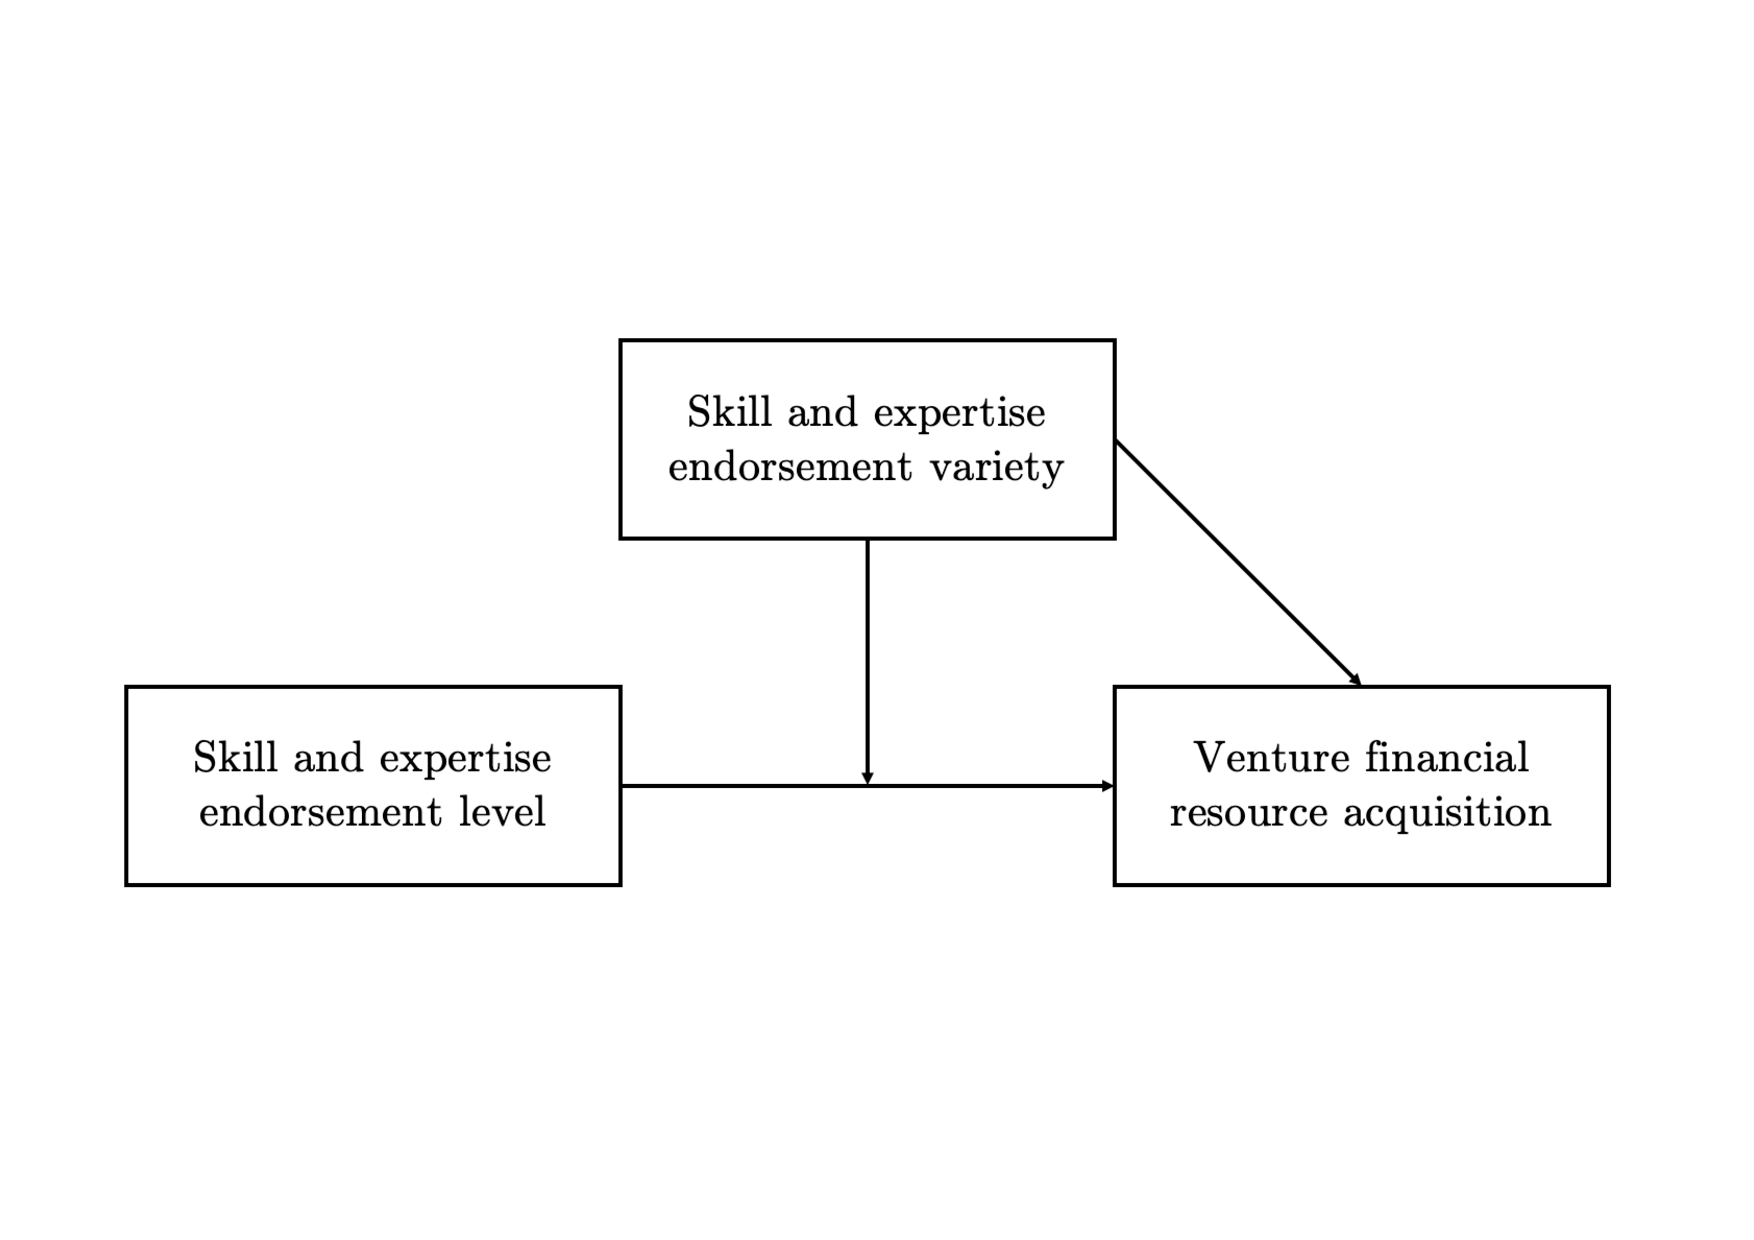
\includegraphics[width=\linewidth, scale=0.5]{model.pdf}
  \caption{Research Model}
  \label{Figure1}
\end{figure*}

\section{Research method}

\subsection{Data sources, collection process and sample selection}

To test our hypotheses, we constructed a dataset incorporating information at both organizational and individual levels of start-up teams. Table 1\label{table1} lists our empirical variables, definitions, and sources. Table 2\label{table2} provides the general statistics and distribution across sectors. Table 3\label{table3} provides the descriptive statistics of the fundraising activities of the 439 digital new ventures in our sample. We detail the collection process below. \\

INSERT TABLES 1, 2 AND 3 HERE. \\

First, we draw on Crunchbase, and BPI France databases as a starting point. The first database follow the evolution of global firms benefiting from venture capital financing. The second is a French state database that lists French-based innovative firms. These databases provide information on the firm’s headquarters, founders’ names, fundraising activity, business models, and date of foundation. We collected this data in March 2020 and kept firms that (i) were founded between 2011 and 2018, (ii) had their headquarters in the Metropolis of Greater Paris (France), (iii) were independent (no subsidiaries), (iv) operated in business-to-business markets and (v) used a scalable business model in the digital industry. From these filters, we ended up with 439 firms. We study firms with digital business models (i.e., software-as-a-service, marketplaces, and platforms) because they echo the efficient, predictable, and repeatable systems that offer investors new opportunities due to the non-linear revenues of digital technologies \citep{nambisan2017digital}. Unlike traditional software licenses that require installers, scalable business models are hosted in the cloud, require little infrastructure, are searchable using a browser, and are delivered over the Internet with or without a subscription-based revenue logic. We also chose the period 2011-2018 because it coincides with the mass adoption of cloud technologies in pre-existing markets. These technologies have revolutionized the software industry in various markets, such as supply chain, financial, accounting, human resources, or customer relationships, making it a topic of interest in various industries. From 2016 to 2020, software-as-a-service, marketplaces, and platforms firms accounted for 55\% of the total amount raised in France, 75\% of French fundraising rounds in Paris, and more than 85\% of the value (BPI, 2020). Furthermore, we chose the Metropolis of Greater Paris (France) because it is a significant global city with labor and financial capital pools and proximate clients. The Metropolis of Greater Paris’ financing and business landscape, especially its venture capital market, is one of Europe’s largest, most structured, and most dynamic one even though characterized by tight links between firms and the state and by powerful elite networks \citep{milosevic2018skills}.

Secondly, we use LinkedIn to collect human capital data of all the founders who worked in these 439 digital firms, representing a total of 1341 individuals. LinkedIn provides granular information on individuals’ professional trajectories and users have an incentive to keep their profiles current since the website is valuable for professional networking: many employers use it to recruit new employees, either by posting job ads or through direct headhunting. While job experience is an indicator frequently used in entrepreneurship studies as a predictor for firm performance (see e.g., \citet{colombo2005founders} or \citet{delmar2006does}), skill endorsement (i.e. skills endorsed and validated by peers on LinkedIn) is a socially constructed online reputation and is a way of self-presentation through which job seekers brand themselves to potential recruiters \citep{rapanta2017linkedin} considered as a piece of valuable information for entrepreneurial studies. Indeed, using skill endorsements data has proven its relevance in recent entrepreneurship studies because it provides detailed individual-level human capital data not available through more traditional sources. For example, \citet{reese2020should} use LinkedIn information about founders, especially their “skills and endorsements” section, to measure founders’ human capital and \citet{sako2020scaling} used LinkedIn “skill endorsement” section too in order to identify the skills of individual start-ups founders. Table 4\label{table4} list the descriptive statistics of all variables (means, std dev, min, max). \\

INSERT TABLE 4 HERE.

\subsection{Data variables}

\subsubsection{Dependent variables}

Our main dependent variable is the amount of funds received by start-ups from external investors in the first round of financing. Receiving funding from an investor is an important predictor of a firm's future survival and growth \citep{beckman2007early}, and inadequate financial resources are frequently cited as the main cause of the failure of new ventures at the start of their life cycle \citep{franke2008venture, eddleston2016you}. In line with previous studies, we use the logarithm of the first round of funding (\textit{log fundraising}) for OLS linear regression. This variable ranges from 0 to a maximum value of 16,524.

\subsubsection{Independant variables}

The main independent variables are \textit{Skills level} and \textit{Skills field variety}. Methodologically speaking, to develop these two variables, we underwent two phases of data pre-treatment.

In the first phase, using the start-up teams online skill endorsement data from LinkedIn \citep{rapanta2017linkedin}, we assigned a score to each team members in the dataset for six functional areas, namely Finance, Product, Development, Management, Marketing, and Entrepreneurship. To create the six functional areas, we employed a bottom-up hierarchical clustering approach with Kruskal's minimum spanning tree algorithm \citep{kruskal1956shortest}, taking into account the occurrences and co-occurrences of skills endorsement among individuals. Therefore, the similarity between any pair of endorsed skills is naturally defined as "intersection over union". Consequently, we determined an individual's affinity to any skill cluster in the tree by measuring the skills that individuals share. In other words, instead of assigning an individual to the cluster with the highest affinity (hard clustering) that would not account for their versatility, we describe an agent by their set of affinities to the skills of interest (fuzzy clustering). This supervised machine learning model is not new and is frequently used in entrepreneurship and management studies \citep{kaushal2021artificial}. In the second phase, we followed the practices of entrepreneurship studies and standardized the scores of each individual to make them comparable across an ordinal variable \citep{harrison2007s}. Specifically, we assigned a ranking to the 1341 individuals from the 439 start-up teams for each functional area based on 10 quantiles, where the 0th quantile represented the lowest level and the 9th quantile represented the highest level of skill endorsement. We developed this variable as an ordinal one, as we contend that for each degree of online endorsement achieved, there is a commensurate effect on the ability to obtain financial resources. Thus, each level corresponds to an incremental advantage for start-ups seeking to secure funding.

From the pre-treatment data process used to generate individual scores, we now possess the necessary raw material to compute firm-level scores for \textit{Skills level} and \textit{Skills field variety}. To measure the start-up team's \textit{Skills level} score, we assigned the highest median score in the six functional areas associated with any of its founders. To measure the start-up team's \textit{Skills field variety} score, we assigned a variable that captures the number of different fields of expertise of its founders. Following \citet{harrison2007s}, we interpret diversity as \textit{variety} defined as \textit{the composition of differences in skills among agents of a unit member}, in this case being the start-up team. Concretely, we compute the variable score based on Blau's index, where the variable is equal to $1-\sum p_k^2$ where $p$ is the proportion of unit members in $k$th category, ranging from zero to $k-1/k$.

\subsubsection{Control variables}

Traditional controls are used to measure entrepreneurs' human capital quality-signals effects.

First, the variable \textit{Previous Prestigious University} was included to take into account the institutionalized cultural capital of the start-up teams members, as defined by \citet{bourdieu1979distinction}. The presence of such capital allows to transmit a quality signal to investors and is thus considered an important factor for start-up teams success. For example, \citet{ferrary1999confiance} empirically demonstrated that degrees from first-plan institutions contribute to quality-signals. In more details, the this variable is constructed from a combination of the top 10 universities worldwide (ARWU 2022 ranking) and the best French business and engineering schools (Figaro Etudiant Ranking 2023). ARWU is not suitable for capturing the entrepreneurial elite graduated in France, due to the weight and attractiveness of French "Grandes Ecoles", poorly represented in ARWU-type international rankings based on Clarivate bibliometric data. The student Figaro ranking integrates the quality of faculty recruitment, relations with industry, and the salary of graduate students.

Second, we use \textit{Previous Founding Experience} to control the number of firms previously founded by the individuals. Indeed, a more extensive entrepreneurial experience can increase investor confidence, send a signal of competence, and have an impact on the amount of raised funds \citep{hsu2007experienced}.

Third, we control for \textit{Previous Working Experience} to determine whether a start-up team member had any significant prior professional experience. Indeed, using human capital and signaling theory, \citet{subramanian2022backing} investigated whether and how founders' human capital characteristics affect early-stage venture capital investment. They concluded that founders with extensive professional working experience attract higher initial investments than other founders.

Fourth, we control for \textit{Previous Ph.D Degree} as teams founded by Ph.D. holders are more likely to receive funding and higher valuations, suggesting a signal effect \citep{hsu2007experienced}.

Fifth, we use \textit{New Venture Age} to control for the time in years since the founding date of a new venture to incorporate a for new ventures' stage of development.

Sixth, we controlled for the \textit{Team size} as a larger start-up team may naturally have more skill endorsements simply due to the greater number of individuals. Therefore, controlling for team size can help isolate the specific effect of skill endorsements on early-stage venture funding. Furthermore, investors often consider team size as one of the factors in their investment decisions. Larger teams may be perceived as more capable in terms of delivering on their proposed business plans \citep{harrison2007s, williamsky1998demographyand}.

Lastly, as there can be confounding effects related to industry conditions in which start-ups operate, we controlled for the \textit{Industry} variables fixed effects. In more details, 11 industry dummies were included which take value 1 if the firm is operating in i) Business Intelligence Analytics, ii) Customer Relationship Management, iii) Developers Software Infrastructure, iv) Education Human Resources, v) Finance Legal Insurance, vi) Healthcare, vii) Logistics Supply Chain, viii) Marketing and Media ix) Productivity Collaboration, x) Real Estate Construction xi) Retail Ecommerce.

\subsubsection{Models}

To test the predictions of our model, we ran an OLS linear regression with the logarithm of the first round of funding (\textit{log fundraising}) as dependent variable. Correlations among the variables are reported in Table 5\label{table5}. The statistical analyses were conducted with Statsmodels Release 0.13.0. The package is released under the open source Modified BSD (3-clause) license \citep{seabold2010statsmodels}. In the following subsection, the dependent, independent, and control variables are introduced. \\

INSERT TABLE 5 HERE.

\section{Analyses and results}

As a first step, we ran an OLS model whose results are reported in Table 6\label{table6}. Model 1 includes only control variables; Model 2 contains only the first independent variable; Model 3 contains only the second independent variable; Model 4 contains the two independent variables; Model 5 comprises the full model with all the independent and moderating variables. We have also controlled for potential multicollinearity problems through a VIF test \citep{james2013introduction}, and no issues of that nature are present. \\

INSERT TABLE 6 HERE. \\

In our first hypothesis, we propose that start-up teams with greater skills endorsement levels will get more fundings from investors. Based on the econometric outcomes presented in table 6, the \textit{Skills level} variable in relation to the natural logarithm of funds demonstrates a positive and highly noteworthy value in Model 2 (p $<$ 0.01), Model 4 (p $<$ 0.01), and Model 5 (p $<$ 0.01). Hence, we validate Hypothesis 1.

Subsequently, in our second assumption, we posited that \textit{Skills field variety} among start-up team members would inspire more optimistic investor expectations concerning the future success of a start-up due to a range of mindsets, superior problem-solving abilities, greater social networks, and a higher probability that diverse organizational tasks would be competently executed. Thus, in our second hypothesis, we posited that diversity of skills fields among start-up team members would result in an increased capacity to obtain funding. As the \textit{Skills field variety} coefficient is positive in model 3 and 4 but very significant only in Model 5 (p $<$ 0.01), we find only partial support for Hypothesis 2.

Lastly, we developed a negative moderating effect of \textit{Skills level} on the relationship between \textit{Skills field variety} and funds raised by the start-up team. In order to arrive at this reasoning, we put forth the notion that team members in a start-up with advanced levels of skill are subject to cognitive inflexibility. Therefore individuals may struggle to interact effectively with other team members whose mental models differ from their own. Therefore, we conjectured that team members with advanced proficiency may have lower chances of providing constructive inputs to the start-up if their peers possess varied skill sets. Thus, we postulated that investors might show a diminished inclination to invest in start-ups where the members possess both extensive proficiency and a wide range of skill and expertise fields. The interaction term between \textit{Skills level} and \textit{Skills field variety} has negative and significant coefficients (p $<$ 0.01) in Model 5, the comprehensive model, thereby providing support for Hypothesis 3.

As a second step, we also estimated a logistic regression as a second regression model in which the dependent variable is a binary (\textit{Fundraising}), since it has been widely used in recent entrepreneurial finance research studies \citep{ahlers2015signaling, islam2018signaling}. Again, Model 1 includes only control variables; Model 2 contains only the first independent variable; Model 3 contains only the second independent variable; Model 4 contains the two independent variables; Model 5 comprises the full model with all the independent and moderating variables. Results are reported in Table 7\label{table7}.

INSERT TABLE 7 HERE. \\

The econometric analysis of the logit regression reveals that the \textit{Skills level} variable exhibits a positive and statistically significant value in Model 2 (p $<$ 0.05), Model 4 (p $<$ 0.05), and most notably in Model 5 (p $<$ 0.001). These findings lend credence to Hypothesis 1.

As per Hypothesis 2, we proposed that \textit{Skills field variety} would catalyze the fundraising process. While the \textit{Skills field variety} coefficient displays a positive orientation in Model 4, it only achieves significance in Model 5 (p $<$ 0.05), implying a partial endorsement of Hypothesis 2.

Lastly, we surmised a counteractive role of the \textit{Skills level} in the association between \textit{Skills field variety} and successful capital acquisition. Our assumption finds support in Model 5, where the interaction term between \textit{Skills level}and \textit{Skills field variety} reveals a negative and significant coefficient (p $<$  0.05), thus supporting Hypothesis 3.

\section{Robustness tests}

We performed several robustness tests to ensure the quality of the analysis.

\textit{Corrected Blau index:} as varying group sizes in a sample affect the most common measures of group diversity \citep{biemann2010size}, we use an alternative formula to get an unbiased estimation of within-group variety ($1 - \sum(N_i*(N_i - 1))/(N*(N - 1))$, where $N_i$ is the absolute frequency of group members in the ith category and N is the total number of group members). Results remain consistent.

\textit{Huber-White test:} we utilized this test for heteroscedasticity using the $het_white$ function of Statsmodels Release 0.13.0. \citep{seabold2010statsmodels}. In our case, the p-value for the White test is 0.36. Consequently, we cannot reject the null hypothesis that the errors are homoscedastic. This infers that based on the test's results, there's insufficient evidence of heteroscedasticity in our data.

\textit{Kruskal's minimum spanning tree algorithm:} there might be room for further discourse about the classification of skills into functional domains, specifically about the relevance of bottom-up hierarchical clustering with Kruskal's algorithm \citep{kruskal1956shortest}. Certainly, certain skills, like entrepreneurship, might be more or less pivotal for different start-up teams. We executed the regressions and assessments using different skills classifications, and the primary findings remain consistent.

\textit{Skills level scores:} finally, we also allocated the highest maximum and mean scores of skills level in the six associated functional areas to any of its founding members to the start-up team. The outcomes derived from utilizing alternate estimators align reasonably well with those shown here and can be provided by the authors upon request.

\section{Discussion}

Research has highlighted the complexity of the effects of start-up team composition on investors' evaluations \citep{cooper1994initial, ghassemiautomated}. Prior studies have found that individual qualities of founding members, such as their education, work experience, and prior entrepreneurial endeavors \citep{shane2002network, hsu2007experienced}, as well as their social capital - the direct or indirect relationships that founding members have with investors, corporate partners, and other entities \citep{shane2002network, hsu2007experienced, huang2017resources} - act as signals of venture quality and are therefore determinants of financial resource acquisition. However, this approach is problematic as investors now use a variety of other signals to assess the relevance of investing in a start-up team \citep{banerji2019startup, mollick2014dynamics, courtney2017resolving}. Recent research has identified online skills endorsement data \citep{gasiorowski2022pay, perez2016endorsement, wu2018analysis} as valuable information for entrepreneurial studies and a reliable criterion for judging an individual's knowledge \citep{rapanta2017linkedin, reese2020should, sako2020scaling}. However, the potential signaling effects of online skills endorsement data on early-stage resource acquisition have been overlooked in the literature. This study aims to address this gap by examining its role in resource acquisition during the early stages of entrepreneurship. Drawing on the theory of signaling, we explore how the social construction of peer-reviewed measures of professional capabilities can influence the ability of start-up teams to acquire financial resources from investors.

This study is motivated by the lack of research on human capital at multiple levels. One issue is the strong bias towards the individual level in previous research \citep{marvel2016human}, with little consideration given to start-up teams and potential inter-individual synergies \citep{knight2020start, sundermeier2022entrepreneurial}. Moreover, previous empirical studies did not engage efforts into assessing how online endorsement skills level, and skills field variety metrics within a start-up team can influence a firm's success in a digital context. Therefore, this article aims to examine these two metrics together, focusing on the dynamics of early-stage start-up teams and how these characteristics relate to the proper operation of the structure. Furthermore, previous empirical studies often used raw measures of human capital, such as years of education, entrepreneurial experiences, or professional experiences, leading to insufficient precision of independent variables used to represent the variables of outcome of human capital \citep{harrison2007s}. Using a sample of 439 digital new ventures in the greater Paris, we demonstrate that, investors favor start-up teams that have (i) either a high level of skills endorsement, (ii) either a high level of variety of skills endorsement, but not both at once. Because of this, start-up teams that contain highly skilled individuals in related fields, i.e., the variety of their skills is low, receive more financial resources.

This paper contributes to the existing literature on entrepreneurship and new venture financing. First, we extent the entrepreneurship literature by providing a new approach to examining the signaling role of start-up team composition, which evaluates both proficiency level and variety of skills based on online endorsement scores. Our approach focuses on the 'outcomes of human capital' (i.e. knowledge, skills and abilities) as a complementary measure to those related to 'investment in human capital' such as education and experience. Second, while many empirical studies looking at how start-up teams' composition affects investors' evaluations focused on indicators such as education \citep{franke2008venture}, entrepreneurial experience \citep{beckman2007early}, industry experience \citep{becker2015new}, or leadership experience \citep{hoenig2015quality}, this article adopt a skill-based approach and derived an outcome-based human capital indicator based on skills endorsement data which is considered a more direct measure of human capital and as one way of analyzing how skills affect firms' performance in a digital environment \citep{marvel2016human}. To do so, we make use of CrunchBase and LinkedIn and demonstrate the value of the data for research to understand the dynamics of signals in entrepreneurship literature. We acknowledge that the public nature of LinkedIn skill endorsements and the elements of performativity and reciprocation inherent in them may introduce potential bias. However, we posit that despite this potential bias, the use of these endorsements as a measure of skill diversity remains valid given their wide acceptance and usage in the professional world.

Nonetheless, our study is not without limitations, paving the way for future research opportunities. For instance, it would be beneficial to identify online skills endorsement effects on dependent variables such as start-ups' innovation performance over the life-cycle of the organization \citep{knight2020start}. Additionally, a larger sample size from different geographies or sectors could be used to augment the generalizability of the findings. Finally, an examination of the impact of online skills endorsement on funds raised in later stages of fundraising, and an effective measurement of the number of conflicts that arise in each start-up depending on its group composition, could enhance our understanding of the significance of group dynamics in signaling trust to investors.

%First, our findings offer fresh avenues for reflection on the composition of start-up teams and the signal generated among investors. Indeed, past empirical studies have long focused on one of the two dimensions of start-up teams' skills. On the one hand, they either focus on their proficiency level, referring to the novice vs. expert, operationally measured by years of experience. On the other hand, they focus on the level of skills' variety, referring to the specialist vs. generalist and operationally measured by the Hirschman or Blau Index). However, when separated, a firm's success is not explained by either of these two dimensions. Furthermore, not only do some levels of skills only apply to some contexts, but certain levels of variety of skills only apply to some contexts. Indeed, the digital context, in contrast to the industrial context, is governed by other social and technological specificities that require different signals. We suggest a methodology in which we assess these two aspects jointly in a digital context.

%Therefore, we derived an outcome-based human capital indicator based on skills and expertise endorsement data which is considered a more direct measure of human capital and as one way of analyzing how skills affect firms' performance in a digital environment \citep{marvel2016human}.

%Recent empirical studies support the idea that multiple forms of variety and organizational performance positively affect firm performance \citep{zhou2015entrepreneurial}.

%According to the literature, there are two types of variety: surface-level differences (e.g., race, ethnic origin, age, etc.), and deep differences (e.g., education, skills, capacities, attitudes and personalities)

%resource-based view of the firm that has become one of the most prominent theoretical perspectives in strategic management (Wernerfelt, 1984; Barney, 1991; Teece, Pisano Shuen, 1997; Rosenkopf Nerkar, 2003; Ahuja Katila, 2004). According to this view, which goes back to the work of Penrose (1959), firms differ in their resource positions and it is such resource heterogeneity that forms an important source of performance differences across firms.

%Since Harrisson : a second theoretical perspective draws from ecological and cognitive models of variation, selection, and retention (e.g., Campbell, 1960) and the cybernetic principle of requisite variety (Ashby, 1956) to highlight the benefits of heterogeneity in information resources. This perspective suggests that variety of attributes such as functional background, tenure, and range of network ties may enrich the supply of ideas, unique approaches, and knowledge available to a unit, enhancing unit creativity, quality of decision making, and complex performance (Williams & O’Reilly, 1998).

% Definition of startup team : Two or more individuals who jointly establish a business in which they have an equity (financial) interest. These individuals are present during the pre-start-up phase of the firm, before it actually begins making its goods or services available to the market.” (Kamm et al., 1990: 7)

%Initial Founding Team Examples: Jung et al. (2017, Study 1); Gray et al. (2019); Powell & Baker (2017)
%start-up team composition, which consistently arose in research on finance (e.g., Bernstein et al., 2017), strategy (e.g., Beckman, 2006), and group dynamics (e.g., Jung et al., 2017).

%there is “no clear relationship” (Klotz et al., 2014: 247), that the literature is “in- conclusive” (Zhou & Rosini, 2015: 33), and that “conflicting results in the literature create uncertainty as to whether and to what extent these characteristics relate to new venture performance” (Jin, Madison, Kraiczy, Kellermanns, Crook, & Xi, 2017: 744).

%A consensus in the entrepreneurial literature emphasize the crucial role of external financial resources for new ventures survival and growth \citep{cooper1994initial}. Indeed, as start-up teams frequently need cash flow to cover the upfront development costs that help to enrich their activities, obtaining external funding is a challenge that cannot be overlooked, especially during the early stages. Whereas early stages external financial resources nature are multiple (see \citet{drover2017review} or \citep{klein2020start} for a review), the main focus of past research on the financial side of start-up teams has been the acquisition of capital from external investors who grant financial capital in exchange for a share of the ownership of the firm. However, acquiring external resources is tought \citep{gompers2010performance}. New ventures gain access to external resources when they can show investors that they have the potential to successful serve a market in the future. From an investor's perspective, investing in an early-stage firm is extremely risky because of the lack of track record of the founding teams or historical financial results and several experiences have shown that it is tough to predict which teams will win \citep{ghassemiautomated, duhigg2016google}. Then, to limit information asymmetries, investors carry out due diligence and base their investment decision on quality-signals \citep{spence1978job, ko2018signaling}. In this regard, signaling theory is appropriate to explain the phenomenon of provisioning resources to new ventures. Signaling theory is especially appropriate for new ventures in new or emerging industries, where established business models or key success factors are not known such as digital context \citep{nambisan2017digital}.

%First, our findings offer new avenues for reflection on the human capital composition of start-up teams and the signal generated among investors. Indeed, past empirical studies have long focused on one of the two dimensions of start-up teams' skills \citep{harrison2007s}. On the one hand, they either focus on their proficiency level, referring to the novice vs. expert, operationally measured by years of experience. On the other hand, they focus on the level of skills' variety, referring to the specialist vs. generalist and operationally measured by the Hirschman or Blau Index). However, when separated, a firm's success is not explained by either of these two dimensions. Furthermore, not only do some levels of skills only apply to some contexts, but certain levels of variety of skills only apply to some contexts. Indeed, the digital context, in contrast to the industrial context, is governed by other social and technological specificities that require different signals. We suggest a methodology in which we assess these two aspects jointly in a digital context.

%In conclusion, although the level and variety of start-up teams' human capital have significant implications for the success of firms in their early stages, empirical results suggest that there is a need for new research on the levels and degrees of variety of start-up teams' skills. Examining the internal team configurations of digital start-up teams through the lenses of skills is one way to respond to this call.

%Early on, start-up teams frequently lack the cash flow needed to cover the costs that will later help them develop their technical and commercial activities. In this stage, the start-up teams of digital firms concentrate primarily on searching for an exploitable idea and selecting a coherent digital business model. Getting external funding allows early-stage businesses to surpass the liability of newness and smallness limitations and finance the development of products or services. Even though open-source software tools and cloud computing have proliferated and generally reduced experimentation costs, business founders still incur initial costs, they might benefits from high level and hogh variety.


\clearpage
%References section - bibliography
\bibliography{biblio}
\bibliographystyle{abbrvnat}

\clearpage
\section{Annexes}

%Table 1
\clearpage
\begin{table} [ht]
\caption{Variable definitions and sources}
\scriptsize
\renewcommand{\arraystretch}{1.5}
\begin{tabularx}{\textwidth}{ p{5cm} p{7cm} p{2.2cm} }
\toprule
\multicolumn{1}{l}{Variable name}&\multicolumn{1}{l}{Description}&\multicolumn{1}{l}{Data source}\\
\cmidrule(r){1-3}
\textbf{Dependent variable}& &\\
1. \textit{Capital Raised (log)} & Natural logarithm of the amount of investment provided by external investors in the first round [€] & Crunchbase, BPI \\
\textbf{Independent variables}& &\\
2. \textit{Skills level} & Ordinate variable ranging from 0 to 9 (0= min; 9= max). Each start-up team is assigned the highest median score associated with any of its members & Linkedin\\
3. \textit{Skills field variety} & Blau index on the probability of finding a particular skill in a start-up team among the six fields identified (i.e., Finance, Product, Development, Management, Marketing, Entrepreneurship) & Linkedin \\
\textbf{Control variables}& &\\
\textbf{Human Capital control variables}& &\\
4. \textit{Previous Prestigious University} & Number of graduations from one of the best French business, engineering schools or from the 10 universities worldwide. Each start-up team is assigned the maximum score associated with any of its members & LinkedIn\\
5. \textit{Previous Founding Experience} & Number of unique ventures previously founded or co-founder. Each start-up team is assigned the maximum score associated with any of its members & LinkedIn\\
6. \textit{Previous Working Experience} & Maximum number of years of work experience of a start-up team member. Each  start-up team in our sample is assigned the highest score associated with any of its members & LinkedIn\\
7. \textit{Previous Ph.D Degree} & Number of Ph.D graduations. Each start-up team is assigned the maximum score associated with any of its members & LinkedIn\\
\textbf{New Ventures control variables}& &\\
8. \textit{New Venture Age} & Number of years since new ventures' foundation & Crunchbase, BPI\\
9. \textit{Team size} & Number of start-up team members & LinkedIn \\
10. \textit{Industry} & Eleven industry dummies which take value 1 if the company is operating in i) Business Intelligence Analytics, ii) Customer Relationship Management, iii) Developers Software Infrastructure, iv) Education Human Resources, v) Finance Legal Insurance, vi) Healthcare, vii) Logistics Supply Chain, viii) Marketing and Media ix) Productivity Collaboration, x) Real Estate Construction xi) Retail Ecommerce & Crunchbase, BPI \\
\cmidrule(r){1-3}
\end{tabularx}
\label{table1}
\end{table}

%Table 2
\clearpage
\begin{table} [ht]
\caption{Distribution of sample : digital new ventures by industry classification}
\begin{spacing}{0.75}
\scriptsize
\renewcommand{\arraystretch}{1.5}
\begin{tabularx}{\textwidth}{ p{10cm} p{1.5cm} p{1.5cm} }
\toprule
\multicolumn{1}{l}{Industry}&\multicolumn{1}{l}{Number of firms}&\multicolumn{1}{l}{\% total}\\
\cmidrule(r){2-3}
Business Intelligence Analytics & 38 & 8.7 \\
Customer Relationship Management & 25 & 5.7 \\
Developers Software Infrastructure & 50 & 11.4 \\
Education Human Resources & 59 & 13.4 \\
Finance Legal Insurance & 51 & 11.6 \\
Healthcare & 24 & 5.5 \\
Logistics Supply Chain & 27 & 6.1 \\
Marketing and Media & 56 & 12.8 \\
Productivity Collaboration & 48 & 10.9 \\
Real Estate Construction & 25 & 5.7 \\
Retail Ecommerce & 36 & 8.2 \\
\cmidrule(r){2-3}
Total & 439 & 100 \\
\midrule
\end{tabularx}
\label{table2}
\end{spacing}
\end{table}

% Table 3
\clearpage
\begin{table} [ht]
\caption{Descriptive statistics of fundraising rounds}
\scriptsize
\begin{tabular}{p{3.2cm} p{1.2cm} p{1.2cm} p{1.2cm} p{1.2cm} p{1.2cm} p{1.2cm} p{1.2cm}}
\toprule
Part A : Fundraising rounds per years \\
& & & \multicolumn{5}{l}{Amount in millions of euros} \\
\cmidrule(l){3-8}
\multicolumn{1}{l}{Fundraising years} & \mc{} & \mc{Rounds} & \mc{Mean}
& \multicolumn{1}{c}{Median} & \mc{Min} & \mc{Max} & \mc{SD} \\
\midrule
2011 & & 4 & 0.251 & 0.115 & 0.025 & 0.750 & 0.338 \\
2012 & & 7 & 0.977 & 0.700 & 0.100 & 2.500 & 0.878 \\
2013 & & 19 & 0.611 & 0.200 & 0.060 & 5.000 & 1.114 \\
2014 & & 30 & 0.752 & 0.370 & 0.055 & 8.000 & 1.457 \\
2015 & & 54 & 1.146 & 0.500 & 0.023 & 10.000 & 1.783 \\
2016 & & 56 & 0.942 & 0.400 & 0.060 & 12.000 & 1.689 \\
2017 & & 67 & 1.542 & 0.750 & 0.050 & 10.000 & 2.090 \\
2018 & & 44 & 1.796 & 1.000 & 0.090 & 15.000 & 2.544 \\
2019 & & 38 & 2.044 & 1.500 & 0.250 & 12.000 & 2.131 \\
2020 & & 11 & 2.410 & 1.000 & 0.500 & 14.500 & 4.073 \\
\cmidrule(l){3-8}
Total	& & 330 & 1.247 & 0.600 & 0.023 & 15.000 & 1.027 \\
 & & \\
\end{tabular}
\\
\\
\\
\begin{tabular}{p{3.2cm} p{1.2cm} p{1.2cm} p{1.2cm} p{1.2cm} p{1.2cm} p{1.2cm} p{1.2cm}}
\toprule
Part B :  Fundraising per founding date \\
 & & & \multicolumn{5}{l}{Amount in millions of euros} \\
\cmidrule(l){2-8}
\multicolumn{1}{l}{Founding date} & \mc{Firms} & \mc{Rounds} & \mc{Mean}
& \multicolumn{1}{c}{Median} & \mc{Min} & \mc{Max} & \mc{SD} \\
\midrule
2011 & 27 & 27 & 1.196 & 0.400 & 0.250 & 7.300 & 1.564 \\
2012 & 36 & 29 & 0.834 & 0.450 & 0 & 4.000 & 1.040 \\
2013 & 58 & 49 & 0.775 & 0.250 & 0 & 8.000 & 1.447 \\
2014 & 65 & 49 & 1.415 & 0.300 & 0 & 15.000 & 2.864 \\
2015 & 74 & 55 & 1.141 & 0.400 & 0 & 14.500 & 2.331 \\
2016 & 85 & 67 & 0.067 & 0.500 & 0 & 12.000 & 1.856 \\
2017 & 60 & 35 & 0.679 & 0.215 & 0 & 3.700 & 0.925 \\
2018 & 34 & 19 & 0.828 & 0.550 & 0 & 4.000 & 1.035 \\
\cmidrule(l){2-8}
Total & 439 & 330 & 0.992 & 0.400 & 0 & 15.000 & 0.687 \\
 & & \\
\end{tabular}
\label{table3}
\end{table}

% Table 4
\clearpage
\begin{table} [ht]
\caption{Descriptive statistics}
\scriptsize
\renewcommand{\arraystretch}{1.5}
\begin{tabularx}{\textwidth}{ p{4.9cm} p{1.6cm} p{1.6cm} p{1.6cm} p{1.6cm} p{1.6cm} }
\toprule
\multicolumn{1}{l}{Variables}&\multicolumn{1}{l}{Obs}&\multicolumn{1}{l}{Mean}&\multicolumn{1}{l}{SD}&\multicolumn{1}{l}{Min}&\multicolumn{1}{l}{Max} \\
\cmidrule(r){1-6}
\textbf{Dependent variable} & & & & & \\
\textit{Capital Raised (log)} & 439 & 10.009 & 5.872 & 0 & 16.524 \\
\cmidrule(r){1-6}
\textbf{Independent variables} & & & & & \\
\textit{Skills level} & 439 & 6.215 & 2.186 & 0 & 9 \\
\textit{Skills field variety} & 439 & 0.621 & 0.354 & 0 & 1 \\
\cmidrule(r){1-6}\textbf{Control variables} & & & & & \\
\textbf{Human capital control variables} & & & & & \\
\textit{Previous Prestigious University} & 439 & 0.827 & 0.766 & 0 & 3 \\
\textit{Previous Founding Experience} & 439 & 1.230 & 0.981 & 0 & 4 \\
\textit{Previous Working Experience} & 439 & 16.724 & 8.629 & 1 & 47 \\
\textit{Previous PhD Degree} & 439 & 0.128 & 0.360 & 0 & 2 \\
\cmidrule(r){1-6}
\textbf{Firms control variables} & & & & & \\
\textit{New Venture Age} & 439 & 5.205 & 1.950 & 2 & 9 \\
\textit{Team size} & 439 & 2.590 & 0.785 & 2 & 8 \\
\textit{Business Intelligence Analytics} & 439 & 0.087 & 0.282 & 0 & 1 \\
\textit{Customer Relationship Management} & 439 & 0.057 & 0.232 & 0 & 1 \\
\textit{Developers Software Infrastructure} & 439 & 0.114 & 0.318 & 0 & 1 \\
\textit{Education Human Resources} & 439 & 0.134 & 0.341 & 0 & 1 \\
\textit{Finance Legal Insurance} & 439 & 0.116 & 0.321 & 0 & 1 \\
\textit{Healthcare} & 439 & 0.055 & 0.228 & 0 & 1 \\
\textit{Logistics Supply Chain} & 439 & 0.062 & 0.241	& 0 & 1 \\
\textit{Productivity Collaboration} & 439 & 0.109 & 0.312 & 0 & 1 \\
\textit{Real Estate Construction} & 439 & 0.057 & 0.232 & 0 & 1 \\
\textit{Marketing Media} & 439 & 0.128 & 0.334 & 0 & 1 \\
\textit{Retail Ecommerce} & 439 & 0.082 & 0.275 & 0 & 1 \\
\midrule
\end{tabularx}
\label{table4}
\end{table}

% Table 5
\clearpage
\begin{sidewaystable}
  \caption{Correlation Table}
\renewcommand{\arraystretch}{2.5}
\setlength{\tabcolsep}{2.5pt}
\scriptsize
    \centering
    \begin{tabular}{cllllllllllllllllllll}
    \toprule
        ~ & ~ & 1 & 2 & 3 & 4 & 5 & 6 & 7 & 8 & 9 & 10 & 11 & 12 & 13 & 14 & 15 & 16 & 17 & 18 & 19 \\ \hline
        1 & Capital Raised (log) & 1 & ~ & ~ & ~ & ~ & ~ & ~ & ~ & ~ & ~ & ~ & ~ & ~ & ~ & ~ & ~ & ~ & ~ & ~ \\
        2 & Skills level & 0.142 & 1 & ~ & ~ & ~ & ~ & ~ & ~ & ~ & ~ & ~ & ~ & ~ & ~ & ~ & ~ & ~ & ~ & ~ \\
        3 & Skills field variety & -0.018 & -0.257 & 1 & ~ & ~ & ~ & ~ & ~ & ~ & ~ & ~ & ~ & ~ & ~ & ~ & ~ & ~ & ~ & ~ \\
        4 & Previous Prestigious University & 0.213 & 0.031 & 0.020 & 1 & ~ & ~ & ~ & ~ & ~ & ~ & ~ & ~ & ~ & ~ & ~ & ~ & ~ & ~ & ~ \\
        5 & Previous Founding Experience & 0.124 & 0.151 & -0.079 & 0.065 & 1 & ~ & ~ & ~ & ~ & ~ & ~ & ~ & ~ & ~ & ~ & ~ & ~ & ~ & ~ \\
        6 & Previous Working Experience & 0.073 & 0.260 & -0.144 & -0.046 & 0.163 & 1 & ~ & ~ & ~ & ~ & ~ & ~ & ~ & ~ & ~ & ~ & ~ & ~ & ~ \\
        7 & Previous PhD Degree & 0.005 & -0.148 & 0.080 & 0.089 & -0.025 & 0.052 & 1 & ~ & ~ & ~ & ~ & ~ & ~ & ~ & ~ & ~ & ~ & ~ & ~ \\
        8 & Firm Age & 0.189 & 0.241 & -0.165 & -0.013 & 0.034 & 0.273 & -0.005 & 1 & ~ & ~ & ~ & ~ & ~ & ~ & ~ & ~ & ~ & ~ & ~ \\
        10 & Team Size & 0.088 & 0.180 & 0.168 & 0.163 & 0.152 & 0.156 & 0.016 & -0.122 & 1 & ~ & ~ & ~ & ~ & ~ & ~ & ~ & ~ & ~ & ~ \\
        11 & Business Intelligence Analytics & -0.033 & -0.038 & 0.002 & 0.059 & -0.122 & 0.025 & 0.026 & 0.130 & -0.025 & 1 & ~ & ~ & ~ & ~ & ~ & ~ & ~ & ~ & ~ \\
        10 & Customer Relationship Management & -0.001 & 0.111 & -0.135 & 0.004 & 0.033 & 0.038 & -0.060 & 0.120 & -0.047 & -0.076 & 1 & ~ & ~ & ~ & ~ & ~ & ~ & ~ & ~ \\
        11 & Developers Software Infrastructure & 0.050 & -0.144 & 0.101 & -0.022 & 0.004 & 0.157 & 0.112 & 0.040 & -0.005 & -0.110 & -0.088 & 1 & ~ & ~ & ~ & ~ & ~ & ~ & ~ \\
        12 & Education Human Resources & 0.023 & 0.082 & -0.058 & -0.068 & -0.045 & -0.078 & -0.028 & -0.100 & 0.053 & -0.121 & -0.097 & -0.141 & 1 & ~ & ~ & ~ & ~ & ~ & ~ \\
        13 & Finance Legal Ins"urance & 0.042 & -0.076 & 0.067 & 0.045 & 0.125 & -0.002 & -0.069 & -0.166 & 0.026 & -0.112 & -0.089 & -0.130 & -0.143 & 1 & ~ & ~ & ~ & ~ & ~ \\
        14 & Healthcare & 0.070 & -0.054 & 0.041 & 0.133 & 0.036 & 0.050 & 0.221 & -0.041 & 0.049 & -0.074 & -0.059 & -0.086 & -0.095 & -0.087 & 1 & ~ & ~ & ~ & ~ \\
        15 & Logistics Supply Chain & -0.009 & 0.053 & 0.049 & -0.041 & -0.041 & -0.025 & -0.012 & -0.027 & 0.098 & -0.079 & -0.063 & -0.092 & -0.101 & -0.093 & -0.062 & 1 & ~ & ~ & ~ \\
        16 & Productivity Collaboration & -0.065 & 0.014 & 0.026 & -0.026 & 0.037 & -0.063 & -0.104 & -0.011 & -0.112 & -0.108 & -0.086 & -0.126 & -0.138 & -0.127 & -0.084 & -0.090 & 1 & ~ & ~ \\
        17 & Real Estate Construction & 0.003 & -0.062 & -0.002 & 0.004 & -0.068 & -0.021 & -0.087 & -0.076 & -0.034 & -0.076 & -0.060 & -0.088 & -0.097 & -0.089 & -0.059 & -0.063 & -0.086 & 1 & ~ \\
        18 & Marketing Media & -0.074 & 0.045 & -0.014 & -0.056 & -0.006 & -0.027 & 0.016 & 0.033 & -0.044 & -0.118 & -0.094 & -0.137 & -0.151 & -0.139 & -0.092 & -0.098 & -0.134 & -0.094 & 1 \\
        19 & Retail Ecommerce & 0.011 & 0.079 & -0.100 & 0.013 & 0.031 & -0.038 & 0.009 & 0.131 & -0.055 & -0.092 & -0.073 & -0.107 & -0.118 & -0.108 & -0.072 & -0.077 & -0.105 & -0.073 & -0.114  \\ \hline
    \end{tabular}
  \label{table5}
  \end{sidewaystable}

% Table 6
\clearpage
\begin{table}[!ht]
\scriptsize
    \centering
    \caption{Results of OLS Regression for Signals and Investment Outcome. Log of funds received is the dependent variable of the OLS linear regression.}
    \begin{tabular}{llllll}
        \toprule
        ~ & \textbf{Model 1} & \textbf{Model 2} & \textbf{Model 3} & \textbf{Model 4} & \textbf{Model 5} \\
        Variables & ~ & ~ & ~ & ~ & ~ \\
        ~ & ~ & ~ & ~ & ~ & ~ \\
        \midrule
        ~ & ~ & ~ & ~ & ~ & ~ \\
        Theorical & ~ & ~ & ~ & ~ & ~ \\
        & ~ & ~ & ~ & ~ & ~ \\
        Skill level (SL) & ~ & 0.250* & ~ & 0.265* & 0.547*** \\
        ~ & ~ & (0.139) & ~ & (0.143) & (0.192) \\
        Skill field diversity (SFD) & ~ & ~ & 0.005 & 0.369 & 4.575** \\
        ~ & ~ & ~ & (0.810) & (0.831) & (2.104) \\
        Interaction SL * SFD & ~ & ~ & ~ & ~ & -1.051** \\
        ~ & ~ & ~ & ~ & ~ & (0.484) \\
        ~ & ~ & ~ & ~ & ~ & ~ \\
        Controls & ~ & ~ & ~ & ~ & ~ \\
        & ~ & ~ & ~ & ~ & ~ \\
        Previous Prestigious University & 1.509*** & 1.477*** & 1.509*** & 1.480*** & 1.478*** \\
        ~ & (0.364) & (0.363) & (0.364) & (0.364) & (0.362) \\
        Previous Founding Experience & 0.527* & 0.481* & 0.527* & 0.489* & 0.463 \\
        ~ & (0.286) & (0.286) & (0.287) & (0.287) & (0.286) \\
        Previous Working Experience & -0.008 & -0.021 & -0.007 & -0.020 & -0.020 \\
        ~ & (0.034) & (0.035) & (0.035) & (0.035) & (0.035) \\
        Previous PhD Degree & -0.374 & -0.168 & -0.374 & -0.179 & -0.256 \\
        ~ & (0.780) & (0.787) & (0.783) & (0.788) & (0.785) \\
        Firm Age & 0.689*** & 0.637*** & 0.689*** & 0.638*** & 0.655*** \\
        ~ & (0.152) & (0.154) & (0.152) & (0.154) & (0.154) \\
        Team Size & 0.451 & 0.346 & 0.451 & 0.308 & 0.213 \\
        ~ & (0.363) & (0.367) & (0.370) & (0.377) & (0.378) \\
        Business Intelligence Analytics & -0.741 & -0.521 & -0.741 & -0.549 & -0.650 \\
        ~ & (1.317) & (1.319) & (1.322) & (1.322) & (1.317) \\
        Customer Relationship Management & -0.309 & -0.352 & -0.309 & -0.336 & -0.347 \\
        ~ & (1.466) & (1.462) & (1.468) & (1.464) & (1.458) \\
        Developers Software Infrastructure & 1.231 & 1.613 & 1.230 & 1.555 & 1.578 \\
        ~ & (1.248) & (1.263) & (1.262) & (1.271) & (1.265) \\
        Education Human Resources & 1.298 & 1.269 & 1.298 & 1.261 & 1.320 \\
        ~ & (1.209) & (1.206) & (1.211) & (1.207) & (1.202) \\
        Finance Legal Insurance & 1.350 & 1.583 & 1.349 & 1.537 & 1.478 \\
        ~ & (1.256) & (1.259) & (1.264) & (1.265) & (1.259) \\
        Healthcare & 1.704 & 1.927 & 1.703 & 1.889 & 1.607 \\
        ~ & (1.521) & (1.522) & (1.528) & (1.526) & (1.525) \\
        Logistics Supply Chain & 0.477 & 0.492 & 0.477 & 0.446 & 0.432 \\
        ~ & (1.449) & (1.446) & (1.455) & (1.451) & (1.444) \\
        Marketing Media & -0.610 & -0.564 & -0.610 & -0.594 & -0.625 \\
        ~ & (1.206) & (1.203) & (1.209) & (1.206) & (1.201) \\
        Productivity Collaboration & -0.633 & -0.531 & -0.634 & -0.571 & -0.696 \\
        ~ & (1.249) & (1.247) & (1.255) & (1.252) & (1.247) \\
        & ~ & ~ & ~ & ~ & ~ \\
        Intercept & 3.109*** & 2.261 & 3.107* & 2.018 & 0.481  \\
        ~ & (1.610) & (1.673) & (1.666) & (1.762) & (1.891) \\
        R-squared & 0.119 & 0.126 & 0.119 & 0.126 & 0.136 \\
        R-squared Adj. & 0.086 & 0.091 & 0.084 & 0.089 & 0.097 \\
        Observations  & 439 & 439 & 439 & 439 & 439 \\
        ~ & ~ & ~ & ~ & ~ & ~ \\
        \midrule
    \end{tabular}
    \begin{tablenotes}
      \item[1] SEs are in parentheses
      \item[2] *** p $<$ .001; ** p $<$ .01; * p $<$ .05
\end{tablenotes}
  \label{table6}
\end{table}

% Table 7
\clearpage
\begin{table}[!ht]
\scriptsize
    \centering
    \caption{Results of Logit Regression for Signals and Investment Outcome. Fundraising is the dependent variable of the Logit regression.}
    \begin{tabular}{llllll}
        \toprule
        ~ & \textbf{Model 1} & \textbf{Model 2} & \textbf{Model 3} & \textbf{Model 4} & \textbf{Model 5} \\
        Variables & ~ & ~ & ~ & ~ & ~ \\
        ~ & ~ & ~ & ~ & ~ & ~ \\
        \midrule
        ~ & ~ & ~ & ~ & ~ & ~ \\
        Theorical & ~ & ~ & ~ & ~ & ~ \\
        & ~ & ~ & ~ & ~ & ~ \\
        Skill level (SL) & ~ & 0.105* & ~ & 0.109* & 0.224*** \\
        ~ & ~ & (0.060) & ~ & (0.061) & (0.086) \\
        Skill field diversity (SFD) & ~ & ~ & -0.005 & 0.135 & 1.801* \\
        ~ & ~ & ~ & (0.365) & (0.375) & (0.942) \\
        Interaction SL * SFD & ~ & ~ & ~ & ~ & -0.424* \\
        ~ & ~ & ~ & ~ & ~ & (0.219) \\
        ~ & ~ & ~ & ~ & ~ & ~ \\
        Controls & ~ & ~ & ~ & ~ & ~ \\
        & ~ & ~ & ~ & ~ & ~ \\
        Previous Prestigious University & 0.720*** & 0.705*** & 0.720*** & 0.704*** & 0.709*** \\
        ~ & (0.179) & (0.179) & (0.179) & (0.179) & (0.180) \\
        Previous Founding Experience & 0.187 & 0.167 & 0.187 & 0.169 & 0.176 \\
        ~ & (0.130) & (0.131) & (0.130) & (0.131) & (0.132) \\
        Previous Working Experience & -0.015 & -0.021 & -0.015 & -0.021 & -0.022 \\
        ~ & (0.015) & (0.016) & (0.015) & (0.016) & (0.015) \\
        Previous PhD Degree & -0.140 & -0.071 & -0.140 & -0.074 & -0.105 \\
        ~ & (0.351) & (0.354) & (0.351) & (0.354) & (0.352) \\
        Firm Age & 0.371*** & 0.350*** & 0.371*** & 0.350*** & 0.366*** \\
        ~ & (0.073) & (0.074) & (0.073) & (0.074) & (0.075) \\
        Team Size & 0.246 & 0.202 & 0.247 & 0.187 & 0.156 \\
        ~ & (0.170) & (0.172) & (0.174) & (0.176) & (0.178) \\

        Business Intelligence Analytics & -0.410 & -0.298 & -0.409 & -0.306 & -0.340 \\
         & (0.583) & (0.589) & (0.584) & (0.589) & (0.592) \\
        Customer Relationship Management & -0.131 & -0.128 & -0.131 & -0.122 & -0.083 \\
         & (0.658) & (0.659) & (0.659) & (0.660) & (0.667) \\
        Developers Software Infrastructure & 0.652 & 0.822 & 0.653 & 0.802 & 0.850 \\
         & (0.582) & (0.591) & (0.586) & (0.594) & (0.597) \\
        Education Human Resources & 0.573 & 0.575 & 0.573 & 0.578 & 0.643 \\
         & (0.550) & (0.551) & (0.550) & (0.551) & (0.556) \\
        Finance Legal Insurance & 0.514 & 0.657 & 0.515 & 0.635 & 0.636 \\
         & (0.574) & (0.582) & (0.579) & (0.585) & (0.587) \\
        Healthcare & 0.941 & 1.113 & 0.941 & 1.108 & 1.055 \\
         & (0.784) & (0.800) & (0.785) & (0.801) & (0.809) \\
        Logistics Supply Chain & 0.179 & 0.203 & 0.180 & 0.185 & 0.212 \\
         & (0.648) & (0.652) & (0.650) & (0.654) & (0.658) \\
        Marketing Media & -0.275 & -0.227 & -0.275 & -0.241 & -0.249 \\
         & (0.531) & (0.534) & (0.533) & (0.535) & (0.536) \\
        Productivity Collaboration & -0.306 & -0.255 & -0.305 & -0.271 & -0.304 \\
         & (0.543) & (0.543) & (0.545) & (0.545) & (0.546) \\

        Intercept & -1.989*** & -2.350*** & -1.987*** & -2.428*** & -3.104*** \\
         & (0.743) & (0.773) & (0.762) & (0.804) & (0.884) \\
        Observations  & 439 & 439 & 439 & 439 & 439 \\
        ~ & ~ & ~ & ~ & ~ & ~ \\
        \midrule
    \end{tabular}
    \begin{tablenotes}
      \item[1] SEs are in parentheses
      \item[2] *** p $<$ .001; ** p $<$ .01; * p $<$ .05
\end{tablenotes}
  \label{table7}
\end{table}

% Table 8
\clearpage
\begin{table}[!ht]
\scriptsize
    \centering
    \caption{Main odds Ratio of the Logit regression.}
    \begin{tabular}{llllll}
        \toprule
        ~ & \textbf{Model 1} & \textbf{Model 2} & \textbf{Model 3} & \textbf{Model 4} & \textbf{Model 5} \\
        Variables & ~ & ~ & ~ & ~ & ~ \\
        ~ & ~ & ~ & ~ & ~ & ~ \\
        \midrule
        ~ & ~ & ~ & ~ & ~ & ~ \\
        Theorical & ~ & ~ & ~ & ~ & ~ \\
        & ~ & ~ & ~ & ~ & ~ \\
        Skill level (SL) & ~ & 1.110 & ~ & 1.115 & 0.044 \\

        Skill field diversity (SFD) & ~ & ~ & 0.995 & 1.144 & 6.057 \\

        Interaction SL * SFD & ~ & ~ & ~ & ~ & 0.654 \\

        ~ & ~ & ~ & ~ & ~ & ~ \\

        Intercept & 0.136 & 0.095 & 0.137 & 0.088 & 0.044 \\

        Observations  & 439 & 439 & 439 & 439 & 439 \\
        ~ & ~ & ~ & ~ & ~ & ~ \\
        \midrule
    \end{tabular}

  \label{table8}
\end{table}

\end{document}
